\documentclass{article}
\usepackage{graphicx}
\begin{document}
\section{Izbira metode}
Podatke razdelimo na train in test množico, hiperparametre nastavljamo na train množici, zaradi prekomernega prileganja. Poskusimo nekaj različnih algoritmov, spreminjamo parametre enega po enega: zvišujemo dokler se izboljšujejo z večjimi skoki, potem poskusimo manjše skoke za boljšo oceno. Najboljši rezultat je v RandomForestClassifier (RFC) z 80 sosedi.

Za avtomatiziran pristop preiskusimo tri algoritme: RFC, SVC in kNN. Številske parametre izbiramo enakomerno med smiselnimi vrednostmi, razen za parameter \verb|min_samples_split| (katerega izbiramo logenakomerno) in parameter \verb|gamma| in \verb|C| v SVC (izbiramo lognormalno). Poleg omenjenih nastavljamo v RFC: \verb|n_estimators| (med 32 in 200), \verb|max_depth| (med 2 in 32), \verb|criterion| (med gini, entropy in log\_loss); v SVC: \verb|shrinking| in tip jedra (sigmoid ali rbf); v kNN: \verb|n_neighbors| (med 2 in 256), \verb|weights| (uniform ali distance) in \verb|p| (1, 2, 3 ali 4).

Najboljša konfiguracija je algoritem RFC z \verb|criterion="log_loss"|, \verb|max_depth=7|, \verb|min_samples_split=5|, \verb|n_estimators=127|

Ne razumem navodila za četrto alinejo; konfiguracija, ki jo vrne hyperopt je samo ena. Prilagam slike za različne konfiguracije algoritmov iz (1.1).
\begin{figure}[h!]
    \caption{RandomForestClassifier}
    \centering
    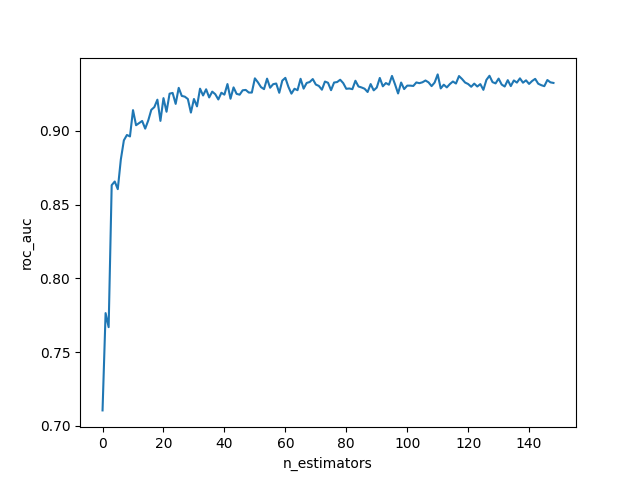
\includegraphics[width=0.8\textwidth]{rfc}
\end{figure}
\begin{figure}[h!]
    \caption{KNeighborsClassifier}
    \centering
    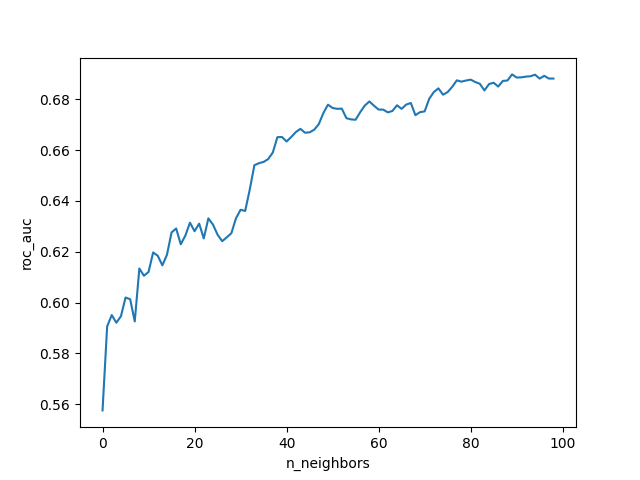
\includegraphics[width=0.8\textwidth]{knn}
\end{figure}
\begin{figure}[h!]
    \caption{SVC}
    \centering
    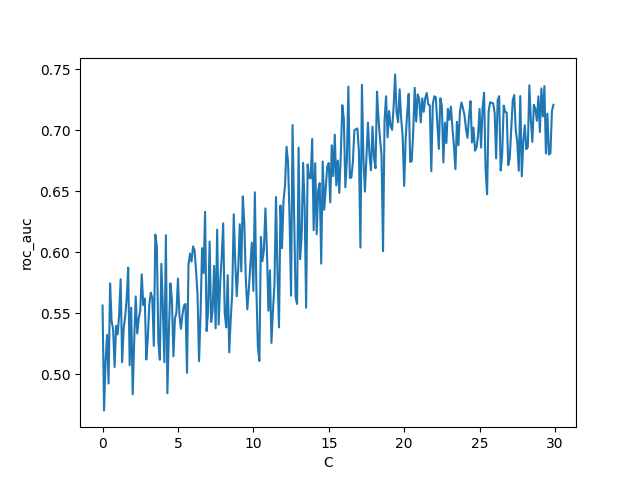
\includegraphics[width=0.8\textwidth]{svc}
\end{figure}
\begin{figure}[h!]
    \caption{MLPClassifier}
    \centering
    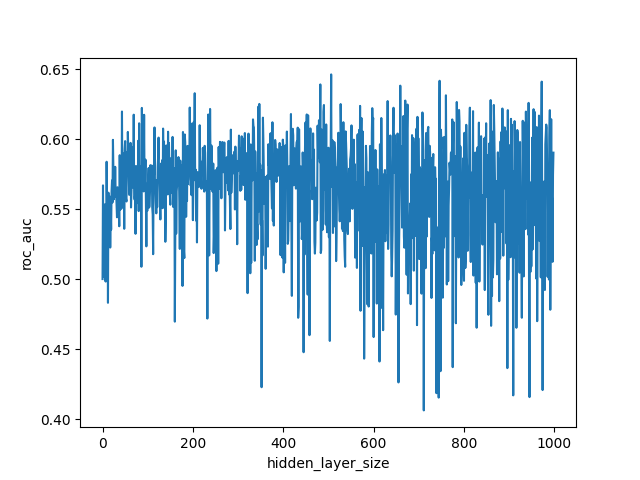
\includegraphics[width=0.8\textwidth]{mlp}
\end{figure}

Iz grafov vidimo, da je RFC daleč najboljši od izbranih algoritmov. Vidimo tudi, da je ročno nastavljena vrednost (80) in vrednost ugotovljena iz metaučenja (127) približno optimalna. Vidimo tudi, da je za SVC potrebno nastaviti $C>20$ in za kNN vsaj $k=80$. Obnašanje enoslojne nevronske mreže je preveč kaotično, da bi iz grafa kaj razbrali vendar vidimo, da se ne nauči dobro.

Na množici za treniranje dobita ročno nastavljanje in hyperopt dobre rezultate (93\% in 93.8\%), izbrali bi hyperopt zaradi malo boljše natančnosti. Na testni množici delata podobno dobro (93\% in 92.2\%), vendar opazimo, da je ročno nastavljanje bilo uspešnejše (izključimo naključnost tako, da povprečimo s 100 različnimi \verb|random_state|), vendar se ne moremo premisliti zaradi prekomernega prileganja.
\begin{figure}[h]
    \caption{roc\_auc za ročno, hyperopt in openml z različnimi naključnimi stanji}
    \centering
    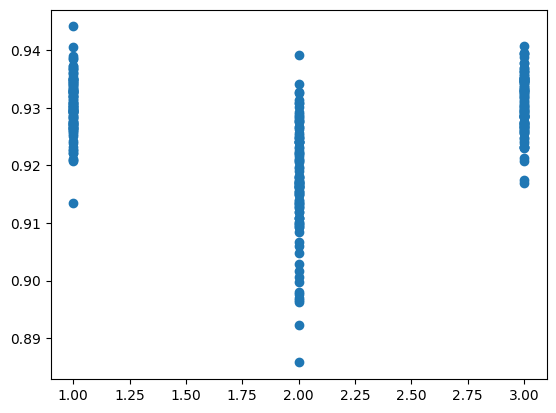
\includegraphics[width=0.8\textwidth]{scores}
\end{figure}

\section{Meta učenje}
Za metaznačilke sem uporabil knjižnico pymfe z skupinami ``general'' in ``info-theory''. To da dovolj dober nabor značilk, da poiščemo bližnje sosede vendar ne vsebuje preveč natančnih metaznačilk, da bi se prilegale samo mojemu naboru podatkov. Namesto ``info-theory'' bi lahko uporabili ``statistical'' ali ``landmarking'', vendar se izkaže, da ne spremeni zaključkov.

Najbližji sosedi so \verb|colleges_usnews|, \verb|pc4| in \texttt{pc4\_seed\_0\_nrows\_2000\_nclasses} \texttt{\_10\_ncols\_100\_stratify\_True}.

Ker je slednji le del \verb|pc4|, za njega ne iščemo kandidatnih algoritmov (saj jih ni objavljenih), uporabimo raje dva algoritma iz \verb|pc4|.

Pri vseh treh sosedih je kandidatni algoritem RFC z dodatnim predprocesiranjem. V prvem je to PCA, v drugem VarianceThreshold in v tretjem StandardScaler. Poskusim tudi združiti pristope (VarianceThreshold+ PCA+ RFC in StandardScaler+ PCA+ RFC). Za najboljšega se izkaže StandardScaler+ PCA+ RFC z ROC\_AUC 93.12\%. To je boljše od hyperopt nastavljanja, torej bi za končni algoritem vzeli tega.

Da dobimo končno natančnost preverimo algoritem na testni množici in dobimo 93.65\% natančnost, kar je najboljše od vseh pristopov. So pa vseeno natančnosti zelo podobne, torej nismo z različnimi pristopi pridobili veliko (prelahko je ročno uganiti dobro konfiguracijo). Predprocesiranje podatkov tudi ni preveč pomagalo, le kake pol procenta, kar pomeni, da so bili podatki že dokaj lepo urejeni vnaprej. Je pa pri tako visoki natančnosti težko najti izboljšave.
\end{document}